\subsection{Formulas: Not \texttt{1+1} but \texttt{=1+1}}


Arithmetic can be done as you would expect, as long as you enter \code{=} and then the formula. Without the equals sign, you will only have text. 

\medskip 

%https://tex.stackexchange.com/questions/493719/approximate-excel-spreadsheet

\begin{center}
\begin{tikzpicture}
\tableur[1]{A}
\celtxt[l,color=red]{A}{1}{=1+1}
\end{tikzpicture} $\rightarrow$  Press enter $\rightarrow$ \begin{tikzpicture}
\tableur[1]{A}
\celtxt[r]{A}{1}{2}
\end{tikzpicture}

\begin{tikzpicture}
\tableur[1]{A}
\celtxt[l,color=red]{A}{1}{1+1}
\end{tikzpicture} $\rightarrow$  Press enter $\rightarrow$ \begin{tikzpicture}
\tableur[1]{A}
\celtxt[l]{A}{1}{1+1}
\end{tikzpicture}
\end{center}






\subsection{Cell References: \texttt{A1}, \texttt{A\$1}, and \texttt{\$A1}}

You can reference the value of another cell using its column and row coordinate. For example, \code{A1} refers to the value in column A, row 1. 

\begin{center}
\begin{tikzpicture}
\tableur[1]{A,B}
\celtxt[r]{A}{1}{2}
%\celtxt[align=left,color=red]{B}{1}{=2}
\celtxt[l,color=red]{B}{1}{=A1 + 2}
\end{tikzpicture} $\rightarrow$  Press enter $\rightarrow$ \begin{tikzpicture}
\tableur[1]{A,B}
\celtxt[r]{A}{1}{2}
\celtxt{B}{1}{4}
\end{tikzpicture}
\end{center}


\subsection{Cell Ranges: \texttt{A1:A2}, \texttt{A:A} and \texttt{A1:B2}}

You can select a range of cells with the mouse or by specifying a range of cell coordinates. When using coordinates, there are three types of ranges you might use. 

\begin{enumerate}
    \item Single column subset, \code{A1:A2}. This will select the cells in column A from row 1 to row 2.
    \item An entire column, \code{A:A}. This will select every cell in column A. 
    \item Rectangular selection, \code{A1:B2}, This will select \code{A1:A2} and \code{B1:B2}. Note, you can use \code{A1:C1} to select all cells in row 1 for columns A-C.
    \item An entire row, \code{1:1}. This will select every row in row 1. 
\end{enumerate}

Selecting a range of cells will be useful later when we use formulas. Note, if you use the reference \code{=A1:B2} by itself, as shown below, you will get back an error because the $2\times 2$ range cannot be inserted into a single cell.\footnote{Use the formula \code{=ARRAYFORMULA(A1:B2)} to copy the contents of \code{A1:B2} to \code{C1:D2}.}
\begin{center}
\begin{tikzpicture}
\tableur[2]{A,B,C}
\celtxt[r]{A}{1}{2}
%\celtxt[align=left,color=red]{B}{1}{=2}
\multiSelect{A-1}{B-2}
%\selecCell{C}{1}
%\celtxt[l,color=red]{C}{1}{=A1:B2}
\cellEntry{C}{1}{=A1:B2}
\end{tikzpicture} 
\end{center}

\subsection{Copying and Pasting Cell References}

To leverage the power of Sheets, you should be copying and pasting your references and formulas as much as possible. There are three types of references that behave differently when copying and pasting. A plain \code{=A1} reference 

\begin{enumerate}
    \item \code{=A1}, relative referencing
    \item \code{=A$1}, mixed referencing where the column is relative
    \item \code{=$A1}, mixed referencing where the row is relative
    \item \code{=$A$1}, absolute referencing
\end{enumerate}

\subsubsection{Relative Column and Row \texttt{=A1}}

\begin{center}
\begin{tikzpicture}
\tableur[2]{A,B,C,D}
\celtxt[r]{A}{1}{1}
\celtxt[r]{B}{1}{2}
\celtxt[r]{A}{2}{10}
\cellEntry{C}{1}{=A1}
\end{tikzpicture} 

$\downarrow$ Paste \code{C1} contents to \code{C2} and \code{D1}.

\begin{tikzpicture}
\tableur[2]{A,B,C,D}
\celtxt[r]{A}{1}{1}
\celtxt[r]{B}{1}{2}
\celtxt[r]{A}{2}{10}

\celtxt[r]{C}{1}{1}
\celtxt[r]{D}{1}{2}
\celtxt[r]{C}{2}{10}
\end{tikzpicture} 
\end{center}


\subsubsection{Relative Column, Absolute Row \texttt{=A\$1}}

The column is relative, because if you paste a reference to cell \code{A1} from \code{C1} to \code{D1}, then the cell reference is essentially updated to \code{B1} so that the movement in columns is reflected in the cell reference. On the other hand, if you paste \code{A1} from \code{C1} to \code{C2}, the row does not update because of absolute reference. The value pasted to \code{C2} will be that found in \code{A1} because there is no column movement and the row is absolute. 

\begin{center}
\begin{tikzpicture}
\tableur[2]{A,B,C,D}
\celtxt[r]{A}{1}{1}
\celtxt[r]{B}{1}{2}
\celtxt[r]{A}{2}{10}
\cellEntry{C}{1}{=A\$1}
\end{tikzpicture} 

$\downarrow$ Paste \code{C1} contents to \code{C2} and \code{D1}.

\begin{tikzpicture}
\tableur[2]{A,B,C,D}
\celtxt[r]{A}{1}{1}
\celtxt[r]{B}{1}{2}
\celtxt[r]{A}{2}{10}

\celtxt[r]{C}{1}{1}
\celtxt[r]{D}{1}{2}
\celtxt[r]{C}{2}{1}
\end{tikzpicture} 
\end{center}

\subsubsection{Absolute Column, Relative Row \texttt{=\$A1}}


The row is relative, because if you paste a reference to cell \code{A1} from \code{C1} to \code{C2}, then the cell reference is essentially updated to \code{A2} so that the movement in rows is reflected in the cell reference. 


\begin{center}
\begin{tikzpicture}
\tableur[2]{A,B,C,D}
\celtxt[r]{A}{1}{1}
\celtxt[r]{B}{1}{2}
\celtxt[r]{A}{2}{10}
\cellEntry{C}{1}{=A\$1}
\end{tikzpicture} 

$\downarrow$ Paste \code{C1} contents to \code{C2} and \code{D1}.

\begin{tikzpicture}
\tableur[2]{A,B,C,D}
\celtxt[r]{A}{1}{1}
\celtxt[r]{B}{1}{2}
\celtxt[r]{A}{2}{10}

\celtxt[r]{C}{1}{1}
\celtxt[r]{D}{1}{1}
\celtxt[r]{C}{2}{10}
\end{tikzpicture} 
\end{center}


\subsubsection{Absolute Column and Row \texttt{=\$A\$1}}

\begin{center}
\begin{tikzpicture}
\tableur[2]{A,B,C,D}
\celtxt[r]{A}{1}{1}
\celtxt[r]{B}{1}{2}
\celtxt[r]{A}{2}{10}
\cellEntry{C}{1}{=A\$1}
\end{tikzpicture} 

$\downarrow$ Paste \code{C1} contents to \code{C2} and \code{D1}.

\begin{tikzpicture}
\tableur[2]{A,B,C,D}
\celtxt[r]{A}{1}{1}
\celtxt[r]{B}{1}{2}
\celtxt[r]{A}{2}{10}

\celtxt[r]{C}{1}{1}
\celtxt[r]{D}{1}{1}
\celtxt[r]{C}{2}{1}
\end{tikzpicture} 
\end{center}